\section{Figures and Tables}

\subsection{TikZ System Diagram}

Figure~\ref{fig:system-architecture} demonstrates a self-contained TikZ figure.
\begin{figure}[H]
    \centering
    \begin{tikzpicture}[scale=0.92, transform shape,
        node distance=0.72cm,
        block/.style={draw, rounded corners, minimum width=2.55cm,
                      minimum height=1.0cm, align=center, fill=blue!5},
        line/.style={-Latex, thick}
    ]
        \node[block] (sensors) {Sensor Array\\$M=4$ channels};
        \node[block, right=of sensors] (adc) {Sampling and\\Calibration};
        \node[block, right=of adc] (dsp) {Covariance and\\DOA Estimation};
        \node[block, right=of dsp] (output) {Health Metric and\\Engineering Report};
        \draw[line] (sensors) -- (adc);
        \draw[line] (adc) -- (dsp);
        \draw[line] (dsp) -- (output);
    \end{tikzpicture}
    \caption{Fictitious smart-sensor-array processing architecture.}
    \label{fig:system-architecture}
\end{figure}

\subsection{Subfigures}

\begin{figure}[H]
    \centering
    \begin{subfigure}[t]{0.47\textwidth}
        \centering
        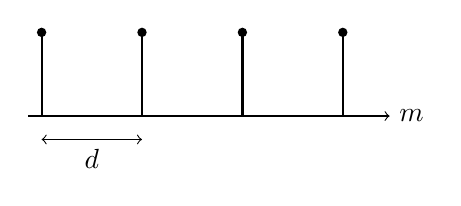
\begin{tikzpicture}[scale=0.85]
            \draw[->] (-0.2,0) -- (5.2,0) node[right] {$m$};
            \foreach \x in {0,1.5,3,4.5}{
                \draw[thick] (\x,0) -- (\x,1.25);
                \fill (\x,1.25) circle (2pt);
            }
            \draw[<->] (0,-0.35) -- (1.5,-0.35) node[midway,below] {$d$};
        \end{tikzpicture}
        \caption{Uniform sensor geometry.}
        \label{fig:sub-array}
    \end{subfigure}
    \hfill
    \begin{subfigure}[t]{0.47\textwidth}
        \centering
        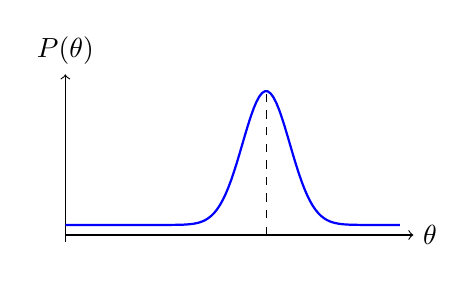
\begin{tikzpicture}[scale=0.85]
            \draw[->] (0,0) -- (5.2,0) node[right] {$\theta$};
            \draw[->] (0,-0.1) -- (0,2.4) node[above] {$P(\theta)$};
            \draw[blue,thick,domain=0:5,samples=120]
                plot (\x,{2*exp(-4*(\x-3)*(\x-3))+0.15});
            \draw[dashed] (3,0) -- (3,2.15);
        \end{tikzpicture}
        \caption{Illustrative spatial spectrum.}
        \label{fig:sub-spectrum}
    \end{subfigure}
    \caption{Example use of the subcaption environment.}
    \label{fig:subfigures}
\end{figure}

\subsection{Robust External-Figure Helper}

The command \verb|\maybeincludegraphics| displays a placeholder rather than stopping
compilation when an expected simulation screenshot has not yet been exported:
\begin{figure}[H]
    \centering
    \maybeincludegraphics[width=0.78\textwidth]{figures/example-simulation-result.png}
    \caption{Missing-file behavior of the robust graphics helper.}
    \label{fig:missing-example}
\end{figure}

\subsection{Technical Tables}

\begin{table}[H]
    \centering
    \caption{Representative design parameters.}
    \label{tab:design-parameters}
    \begin{tabular}{@{}lll@{}}
        \toprule
        Parameter & Symbol & Example value \\
        \midrule
        Operating frequency & $f_0$ & \SI{2.45}{\giga\hertz} \\
        Number of channels & $M$ & 4 \\
        Sensor spacing & $d$ & $\lambda/2$ \\
        Snapshot count & $N$ & 256 \\
        Nominal SNR & $\mathrm{SNR}$ & \SI{10}{\decibel} \\
        \bottomrule
    \end{tabular}
\end{table}

\begin{longtable}{@{}p{0.18\textwidth}p{0.26\textwidth}p{0.46\textwidth}@{}}
\caption{Example verification matrix.}\label{tab:verification-matrix}\\
\toprule
Requirement & Evidence & Acceptance statement \\
\midrule
\endfirsthead
\toprule
Requirement & Evidence & Acceptance statement \\
\midrule
\endhead
Geometry & Figure~\ref{fig:sub-array} & Four uniformly spaced channels are represented. \\
Covariance & Equation~\eqref{eq:sample-covariance} & The estimator uses all available snapshots. \\
Direction estimate & Example spectrum & The dominant peak is reported as the recovered angle. \\
Reproducibility & Appendix~\ref{app:source-code} & The example script and console output are included. \\
\bottomrule
\end{longtable}
